\subsection{Платформа \LB}
\label{sec:technology:logicblox}

В данном подразделе будут рассмотрены основные аспекты разработки приложений на платформе \LB, обзор технологии, архитектуру приложения, а также немного погрузимся в технические аспекты, разберемся в основных отличиях от стандартных приложений.

Первое, с чего следует начать, это с рассмотрения обычной трехслойной архитектуры приложения. При стандартном подходе выделяются Data Store layer (слой базы данных), Business Logic layer (слой бизнес-логики), UI layer (слой представления).

Слой базы данных обеспечивает хранение данных, реализуется в основном средствами систем управления базами данных, подключение к этому компоненту обычно обеспечивается только с уровня сервера приложений. В слое базы данных, как правило, находится не одна база. В большинстве случаев применяются 2 типа: \olap (OnLine Analytical Processing) и \oltp (OnLine Transactional Processing).
\oltp характеризуется большим количеством маленьких транзакций (INSERT, UPDATE, DELETE). Основной упор \oltp систем делается на быструю обработку запросов, управление интегрируемостью данных в мультидоступной среде. Ее эффективность измеряется в количестве транзакций в секунду. В таких базах данные детализированы и схема представляет собой модель сущности (как правило, в 3 нормальной форме).
\olap же характеризуется относительно низкими объемами транзакций. Запросы сами по себе трудоемкие и сложные, часто включают в себя агрегацию. Здесь эффективностью является время ответа на запрос. \olap приложения используются, например, в технологиях Data Mining \cite{olap_and_data_mining}. Такие базы содержат в себе агрегированные, исторические данные.

Приведем ключевые различия между этими видами в таблице \ref{table:technology:logicblox:oltp_olap_diff}:

\begin{longtable}{|>{\raggedright}m{0.2\textwidth}|>{\raggedright\arraybackslash}m{0.35\textwidth}|>{\raggedright\arraybackslash}m{0.35\textwidth}|}
\caption{Ключевые отличия между \oltp и \olap системами \cite{first_course_in_db}}
\label{table:technology:logicblox:oltp_olap_diff}
\centering
	\hline
	\begin{minipage}{1\linewidth}
		\centering Критерий
	\end{minipage} &
	\begin{minipage}{1\linewidth}
		\centering \oltp
	\end{minipage} &
	\begin{minipage}{1\linewidth}
		\centering \olap
	\end{minipage}
	\endfirsthead
	\caption*{Продолжение таблицы \ref{table:technology:logicblox:oltp_olap_diff}}\\
	\hline
	\centering 1 & \centering 2 & \centering\arraybackslash 3\\
	\hline
	\endhead
	\hline
	\centering 1 & \centering 2 & \centering\arraybackslash 3\\

  \hline Источник даных & Операционные данные, сама база является источником & Консолидированные данные, часто содержит в себе несколько \oltp баз \\
  \hline Цель хранения данных & Контроль и выполнение базовых бизнес-задач & Помощь в планировании, решении проблем, поддержка решений \\
  \hline Что является данными & Представляет собой снимок, или срез, постоянных бизнес-процессов & Многоразмерные содержания различных видов бизнес-активностей \\
  \hline Запросы вставки и обновления & Короткие и быстрые вставки и обновления, инициируемые конечным пользователем & Периодические долго выполняющиеся запросы \\
  \hline Запросы & Как правило стандартизируемые и простые запросы. Возвращают небольшие ответы & Часто сложные запросы с агрегацией \\
  \hline Скорость обработки & Быстрая & Зависит от количества используемых данных; скорость запросов может улучшаться с помощью применения индексов \\
  \hline Требования по памяти & Может быть достаточно небольшая, если исторические данные архивируются & Больше, чем в \oltp, из-за структур для агрегации и исторических данных, требует также больше индексов \\
  \hline Дизайн базы & Большая степень нормализованности со множеством таблиц & Не нормализованная с небольшим количество таблиц, имеют схемы звезды \\
  \hline Резервное копирование & Копируется постоянно. Операционные данные имеют решающее значение для ведения бизнеса, их потеря может привести к значительным денежным затратам и юридической ответственности & Вместо регулярных сохранений некоторые среды могут просто перезагружать \oltp данные в качестве метода восстановления \\
	\hline
\end{longtable}

Как правило, программирование в них идет с помощью \sql, PL/\sql, в \olap возможно применение MDX. При текущих высоких нагрузках также возможно использование \nosql, \hadoop кластера и т.д.

Бизнес-логика обычно работает в сервере приложений (если это веб-приложение). В этом слое применяются такие языки, как \java, \csharp, \python, \scala.
Уровень \ui (слой представления) - веб-приложение с \html и \js. Все эти слои представлены на рисунке \ref{fig:technology:logicblox:three_tier_architecture}.

\begin{figure}
	\centering
	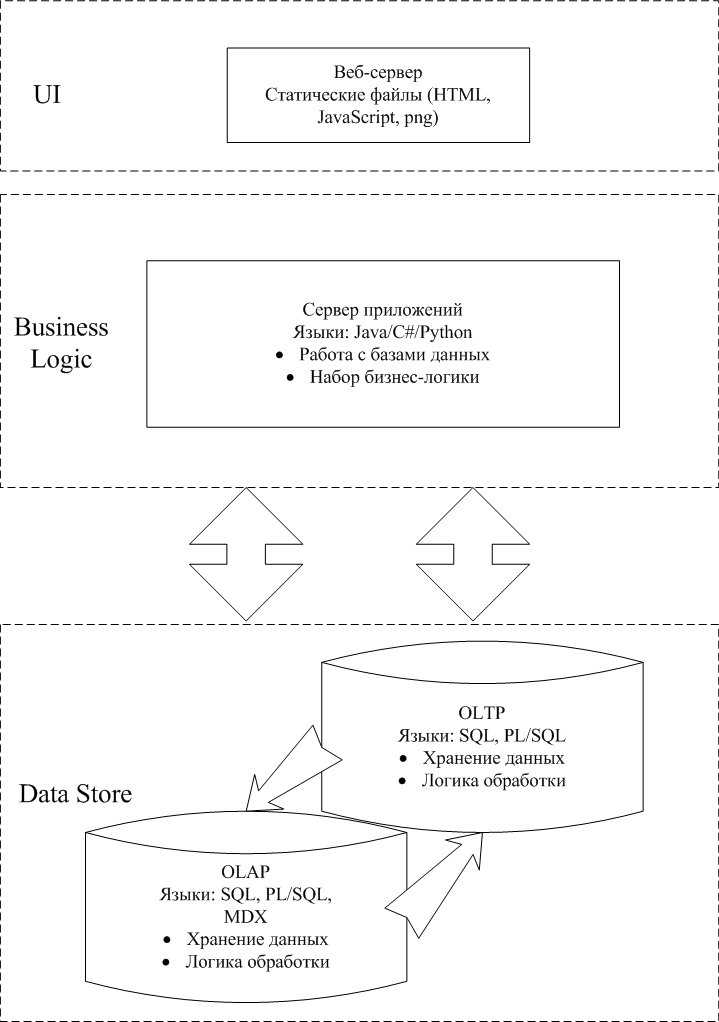
\includegraphics[scale=0.9]{3tier.png}
	\caption{Схема обычного приложения с 3-уровневой архитектурой}
	\label{fig:technology:logicblox:three_tier_architecture}
\end{figure}

При всем этом существует достаточно большое взаимодействие между сервером приложений и уровнем базы данных. Это не всегда тривиальный код, который преобразует схему базы данных между двумя уровнями. В базе данных все хранится в реляционных таблицах, которые нужно трансформировать в используемые компоненты в сервере приложений, или в объекты. Очевидно, ключевой задачей является минимизация движения этих данных, поскольку в большинстве случаев это не только замедляет работу приложения, но также может быть достаточно дорогой операцией. Зачастую накладывается ограничение на используемую память слоя бизнес-логики, поэтому есть пределы сверху на размер информации.

Более того, если в приложении используются как аналитические запросы, так и транзакционные обновления, необходимо учитывать и взаимодействие между самими \olap и \oltp базами данных. Понятно, что они должны быть синхронизируемы между собой, то есть данные должны быть консистентными. Согласно последним исследованиям на данного рода операции отводится свыше 50\% времени работы баз данных.

На момент создания платформы (2000-е гг.) существовали два основных подхода в выборе архитектуры системы базы данных: специализированная и общая. Специализированная предназначена для решения узкопрофильных задач: графы, аналитика, обработка документов и многие другие \cite{one_size_fits_all}. Движущей силой в выборе этого типа является производительность: раз система делает некоторый стандартный набор задач, значит, ее можно хорошо оптимизировать. Так, в сравнении с традиционными \emph{OldSQL} (oldschool) архитектурами, созданными лет 40 назад прирост в производительности может быть 10-100-кратный.

В то же время в последнее время наблюдается тенденция к использованию сложных систем для принятия решений, которые в себе содержат многие из областей, упомянутых в прошлом слайде. Такие приложения подвержены быстрым изменениям, они постоянно улучшаются, растут, поэтому в таких условиях продуктивность программиста становится очень важной и неотъемлемой частью процесса разработки. Идейные вдохновители \LB уверены, что создание такой сложной системы (\emph{hairball}) высокозатратно, а ее поддержка вообще практически невозможна. Такие наблюдения позволяют переосмыслить ценность использования базы данных общего назначения.

Так чем же вызвана такая разница в производительности между архитектурами этих систем? Какими-то фундаментальными причинам? Либо традиционные архитектуры все же не могут извлечь максимум для построения систем общего назначения? Команда разработчиков \LB склонна к последнему мнению. И для своего доказательства они и создали систему базы данных, которая показывает возможность создания приложений без существенных ограничений на производительность и масштабируемость. Исходя из опыта ее использования, цикл разработки менее затратен, эффективен и позволяет сделать поддержку очень легкой.

Чтобы понять более детально, почему именно такое мнение высказывают авторы, давайте разберем на примере смартфона. Этот гаджет был "унаследован” от мобильного телефона, исключительной задачей которого была телефонная связь. Но в последние пару десятков лет смартфон помимо изначальной цели (связи, которую также усовершенствовал, добавив почту, мессенджеры) начал использоваться как музыкальный плеер, как фото/видеокамера, как навигатор, как устройство для игр. Конечно, если сравнивать с цифровой фотокамерой, то качество у смартфона не такое высокое (в среднем), если захотеть поиграть, то лучше использовать компьютер с мощной видеокартой или приставку. То есть рассматривая в отдельности каждые модули, имеющиеся в смартфоне, они уступают целевым аналогам, но кто сейчас не использует смартфон? Для многих людей использование специальных средств (фотоаппараты, мп3-плееры) просто не оправдано, ведь у них есть смартфон. Кроме того, смартфон позволяет не просто снимать на камеру, а еще и посылать сразу же фотографии друзьям, то есть:

\begin{itemize}
	\item налажена интеграция между компонентами;
	\item она значительно удобнее и быстрее в использовании, чем отдельные устройства.
\end{itemize}

Точно такие же идеи заложены и в платформе \LB, поэтому ее называют \emph{smart database}. Ее цель не обойти по производительности специализированные системы, а приблизиться к ним с некоторым небольшим отклонением, но при этом не жертвуя удобством разработки.

В платформе \LB также используется 3-уровневая архитектура, за исключением некоторых ключевых моментов, которые представлены здесь в ином виде. В слое базы данных используется лишь одна база данных вместо нескольких разновидностей. Такая база называется \LB Database, при этом она не построена на основании какой-либо другой (\postgres и т.п.), то есть она разработана "с чистого листа". Благодаря этому она может обрабатывать различные виды нагрузки, которые нужны в рассматриваемой сфере. Объединение всех слоев можно представить рисунком \ref{fig:technology:logicblox:lb_parts_diagram}.

\begin{figure}
	\centering
	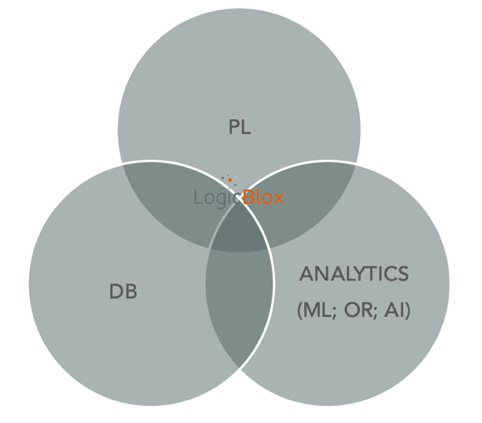
\includegraphics[scale=1]{lb_part_diagram.png}
	\caption{Структура платформы \cite{query_parallel_execution}}
	\label{fig:technology:logicblox:lb_parts_diagram}
\end{figure}

Кроме того, здесь используется новый язык \logiql. Основной целью его разработки были легкость выражения хранения данных, а также логики обработки и логики взаимодействия данных. В платформе \LB слой бизнес-логики предельно прост и тонок, поскольку большая часть логики обработки данных заложена именно в самой базе данных. В большинстве приложений вообще нет слоя бизнес-логики как такового - все выполняется в самой базе. В этом случае отпадает необходимость в трудоемком взаимодействии между этими двумя слоями. Кроме того, любое изменения в схеме базы данных отражается лишь в самой базе - нет нужды отслеживать это изменение в другом слое.

Итак, как итог, можно выделить следующие ключевые факторы в платформе \LB:

\begin{itemize}
	\item включает в себя аналитическую, транзакционную обработку данных, содержит математические оптимизационные алгоритмы;
	\item единый декларативный язык программирования \logiql - не стоит учить несколько различных языков;
	\item нет необходимости отслеживания за консистентностью данных между различными базами данных;
	\item может содержать в себе машинное обучение (для компонента прогноза продаж).
\end{itemize}

Схема приложения \LB представлена на рисунке \ref{fig:technology:logicblox:lb_architecture}.

\begin{figure}
	\centering
	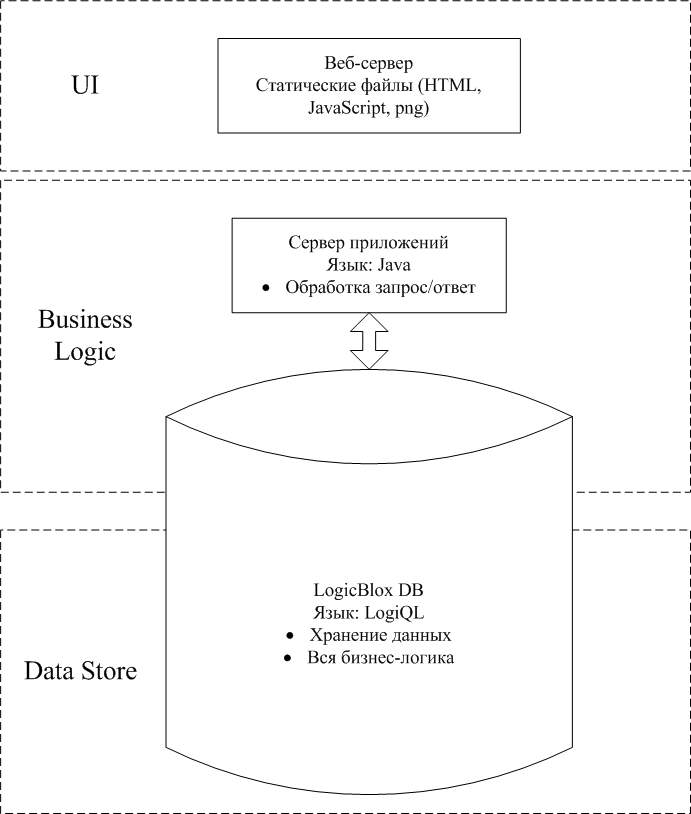
\includegraphics[scale=1]{lb_architecture.png}
	\caption{Схема приложения \LB с 3-уровневой архитектурой \cite{lb_platform}}
	\label{fig:technology:logicblox:lb_architecture}
\end{figure}

Посмотрим на состав самой базы. В ней находится 3 сегмента \cite{lb_db_overview}:

\begin{enumerate}
	\item Определение схемы, как и в других базах данных, с полями, колонками, ограничениями. Пример предикатов:
	\begin{lstlisting}[language=Prolog]
	sales_u(product, store, day, unit) ->
		string(product),
		string(store),
		datetime(day),
		int(unit).

	returns_u(product, store, day, units) ->
		string(product),
		string(store),
		datetime(day),
		int(units).
	\end{lstlisting}
	\item Бизнес-правила:
	\begin{lstlisting}[language=Prolog]
	netsales_u(product, store, day, net) <-
	  sales_u(product, store, day, sls),
	  returns_u(product, store, day, returns),
	  net = sls - returns.
	\end{lstlisting}
	\item Конфигурация сервисов, которые сервер приложений будет использовать для тех или иных целей \cite{query_language_for_smart_db}.
\end{enumerate}
